% Options for packages loaded elsewhere
\PassOptionsToPackage{unicode}{hyperref}
\PassOptionsToPackage{hyphens}{url}
%
\documentclass[
  ignorenonframetext,
]{beamer}
\usepackage{pgfpages}
\setbeamertemplate{caption}[numbered]
\setbeamertemplate{caption label separator}{: }
\setbeamercolor{caption name}{fg=normal text.fg}
\beamertemplatenavigationsymbolsempty
% Prevent slide breaks in the middle of a paragraph
\widowpenalties 1 10000
\raggedbottom
\setbeamertemplate{part page}{
  \centering
  \begin{beamercolorbox}[sep=16pt,center]{part title}
    \usebeamerfont{part title}\insertpart\par
  \end{beamercolorbox}
}
\setbeamertemplate{section page}{
  \centering
  \begin{beamercolorbox}[sep=12pt,center]{section title}
    \usebeamerfont{section title}\insertsection\par
  \end{beamercolorbox}
}
\setbeamertemplate{subsection page}{
  \centering
  \begin{beamercolorbox}[sep=8pt,center]{subsection title}
    \usebeamerfont{subsection title}\insertsubsection\par
  \end{beamercolorbox}
}
\AtBeginPart{
  \frame{\partpage}
}
\AtBeginSection{
  \ifbibliography
  \else
    \frame{\sectionpage}
  \fi
}
\AtBeginSubsection{
  \frame{\subsectionpage}
}
\usepackage{amsmath,amssymb}
\usepackage{iftex}
\ifPDFTeX
  \usepackage[T1]{fontenc}
  \usepackage[utf8]{inputenc}
  \usepackage{textcomp} % provide euro and other symbols
\else % if luatex or xetex
  \usepackage{unicode-math} % this also loads fontspec
  \defaultfontfeatures{Scale=MatchLowercase}
  \defaultfontfeatures[\rmfamily]{Ligatures=TeX,Scale=1}
\fi
\usepackage{lmodern}
\ifPDFTeX\else
  % xetex/luatex font selection
\fi
% Use upquote if available, for straight quotes in verbatim environments
\IfFileExists{upquote.sty}{\usepackage{upquote}}{}
\IfFileExists{microtype.sty}{% use microtype if available
  \usepackage[]{microtype}
  \UseMicrotypeSet[protrusion]{basicmath} % disable protrusion for tt fonts
}{}
\makeatletter
\@ifundefined{KOMAClassName}{% if non-KOMA class
  \IfFileExists{parskip.sty}{%
    \usepackage{parskip}
  }{% else
    \setlength{\parindent}{0pt}
    \setlength{\parskip}{6pt plus 2pt minus 1pt}}
}{% if KOMA class
  \KOMAoptions{parskip=half}}
\makeatother
\usepackage{xcolor}
\newif\ifbibliography
\usepackage{longtable,booktabs,array}
\usepackage{calc} % for calculating minipage widths
\usepackage{caption}
% Make caption package work with longtable
\makeatletter
\def\fnum@table{\tablename~\thetable}
\makeatother
\usepackage{graphicx}
\makeatletter
\newsavebox\pandoc@box
\newcommand*\pandocbounded[1]{% scales image to fit in text height/width
  \sbox\pandoc@box{#1}%
  \Gscale@div\@tempa{\textheight}{\dimexpr\ht\pandoc@box+\dp\pandoc@box\relax}%
  \Gscale@div\@tempb{\linewidth}{\wd\pandoc@box}%
  \ifdim\@tempb\p@<\@tempa\p@\let\@tempa\@tempb\fi% select the smaller of both
  \ifdim\@tempa\p@<\p@\scalebox{\@tempa}{\usebox\pandoc@box}%
  \else\usebox{\pandoc@box}%
  \fi%
}
% Set default figure placement to htbp
\def\fps@figure{htbp}
\makeatother
\setlength{\emergencystretch}{3em} % prevent overfull lines
\providecommand{\tightlist}{%
  \setlength{\itemsep}{0pt}\setlength{\parskip}{0pt}}
\setcounter{secnumdepth}{-\maxdimen} % remove section numbering
\usepackage{bookmark}
\IfFileExists{xurl.sty}{\usepackage{xurl}}{} % add URL line breaks if available
\urlstyle{same}
\hypersetup{
  pdftitle={vignette},
  pdfauthor={Francesca Lo Bianco},
  hidelinks,
  pdfcreator={LaTeX via pandoc}}

\title{vignette}
\author{Francesca Lo Bianco}
\date{2025-07-23}

\begin{document}
\frame{\titlepage}

\begin{frame}
\begin{block}{setting the working directory}
\phantomsection\label{setting-the-working-directory}
\end{block}

\begin{block}{extracting and loading the datasets provvided}
\phantomsection\label{extracting-and-loading-the-datasets-provvided}
gtf\_path \textless-``Homo\_sapiens.GRCh38.111.gtf.gz'' gtf \textless-
read.delim(gzfile(gtf\_path), header = FALSE, comment.char = ``\#'')

unzip(``filtered\_feature\_bc\_matrix.zip'',exdir =
``filtered\_feature\_bc\_matrix'')
\end{block}

\begin{block}{installing DropletUtils to extract the features}
\phantomsection\label{installing-dropletutils-to-extract-the-features}
if (!requireNamespace(``DropletUtils'', quietly = TRUE)) \{
BiocManager::install(``DropletUtils'') \} library(DropletUtils)
\end{block}

\begin{block}{setting the path to matrix folder to read the features}
\phantomsection\label{setting-the-path-to-matrix-folder-to-read-the-features}
matrix\_dir
\textless-``filtered\_feature\_bc\_matrix/filtered\_feature\_bc\_matrix''
sce \textless- read10xCounts(matrix\_dir)
\end{block}

\begin{block}{checking everything}
\phantomsection\label{checking-everything}
sce
\end{block}
\end{frame}

\begin{frame}{1.Gene Annotation: Identify and retain only the
protein-coding genes from the dataset, based on the GTF file.}
\phantomsection\label{gene-annotation-identify-and-retain-only-the-protein-coding-genes-from-the-dataset-based-on-the-gtf-file.}
\begin{block}{creating a table for gtf}
\phantomsection\label{creating-a-table-for-gtf}
gtf
\textless-read.table(gzfile(``C:/Users/Utente/Desktop/magistrale/programming/exam/Homo\_sapiens.GRCh38.111.gtf.gz''),
header = FALSE, sep = ``\t", comment.char =''\#``, stringsAsFactors =
FALSE, quote =''\,``)

head(gtf)
\end{block}

\begin{block}{creating a function to estract the characteristics of the
genes fromthe 9th column}
\phantomsection\label{creating-a-function-to-estract-the-characteristics-of-the-genes-fromthe-9th-column}
library(stringr)

extract\_characteristics \textless- function(attr\_string, key) \{
pattern \textless- paste0(key, '' ``({[}\^{}\textbackslash''{]}+)''\,``)
match \textless- regmatches(attr\_string, regexec(pattern,
attr\_string)) sapply(match, function(x) if(length(x) \textgreater{} 1)
x{[}2{]} else NA) \}
\end{block}

\begin{block}{extracting id and biotype in their column}
\phantomsection\label{extracting-id-and-biotype-in-their-column}
gtf\(gene_id <- extract_characteristics(gtf\)V9, ``gene\_id'')
gtf\(gene_biotype <- extract_characteristics(gtf\)V9,``gene\_biotype'')
\end{block}

\begin{block}{finding the protein coding genes making it searchig in the
gene biotype column}
\phantomsection\label{finding-the-protein-coding-genes-making-it-searchig-in-the-gene-biotype-column}
protein\_coding\_genes \textless- unique(gtf\(gene_id[gtf\)gene\_biotype
== ``protein\_coding''{]})
\end{block}

\begin{block}{creating a matrix only with the protein coding genes}
\phantomsection\label{creating-a-matrix-only-with-the-protein-coding-genes}
filtered\_matrix \textless- sce{[}rownames(sce) \%in\%
protein\_coding\_genes, {]}
\end{block}

\begin{block}{cheking it worked}
\phantomsection\label{cheking-it-worked}
ls() class(sce) dim(sce) dim(filtered\_matrix)
\end{block}
\end{frame}

\begin{frame}{2.Gene Expression Summary:For each cell, calculate the
number of genes with expression ≥3 UMIs. Display the distribution of
these counts using a violin plot.}
\phantomsection\label{gene-expression-summaryfor-each-cell-calculate-the-number-of-genes-with-expression-3-umis.-display-the-distribution-of-these-counts-using-a-violin-plot.}
\begin{block}{calculating the counts to create a sparse matrix}
\phantomsection\label{calculating-the-counts-to-create-a-sparse-matrix}
library(SingleCellExperiment) counts\_matrix \textless- counts(sce)
\end{block}

\begin{block}{selecting only the genes with expression ≥3 UMIs}
\phantomsection\label{selecting-only-the-genes-with-expression-3-umis}
genes\_over\_3 \textless-colSums(counts\_matrix \textgreater= 3)
\end{block}

\begin{block}{checking it worked}
\phantomsection\label{checking-it-worked}
summary(genes\_over\_3)
\end{block}

\begin{block}{getting the ggplot2 library to create the plot}
\phantomsection\label{getting-the-ggplot2-library-to-create-the-plot}
library(ggplot2)
\end{block}

\begin{block}{converting to data frame for plotting}
\phantomsection\label{converting-to-data-frame-for-plotting}
df \textless- data.frame(GenesOver3UMI = genes\_over\_3)
\end{block}

\begin{block}{violin plot}
\phantomsection\label{violin-plot}
ggplot(df, aes(x = ``\,``, y = GenesOver3UMI)) + geom\_violin(fill
=''blue'', alpha = 0.6) + geom\_boxplot(width = 0.1, outlier.shape = NA)
+ labs( title = ``Number of Genes with ≥3 UMIs'', y = ``Genes with ≥3
UMIs'', x = ``\,'' ) + theme\_minimal(12)

\begin{figure}
\centering
\pandocbounded{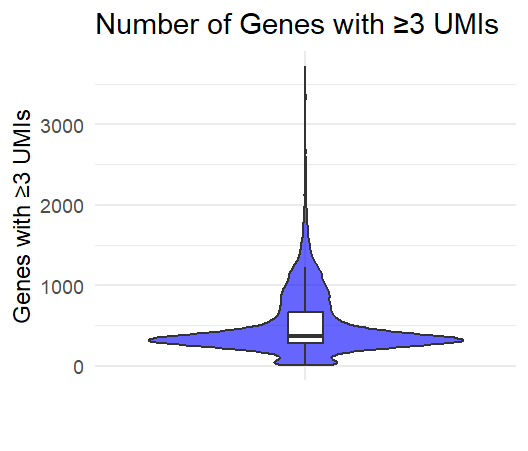
\includegraphics[keepaspectratio]{final violin plot.png}}
\caption{violin plot}
\end{figure}
\end{block}
\end{frame}

\begin{frame}{3.Gene Filtering:Exclude the following gene
categories:Ribosomal proteins, Ribosomal pseudogenes, Mitochondrial
genes. Provide a summary table listing the number of genes removed from
each category.}
\phantomsection\label{gene-filteringexclude-the-following-gene-categoriesribosomal-proteins-ribosomal-pseudogenes-mitochondrial-genes.-provide-a-summary-table-listing-the-number-of-genes-removed-from-each-category.}
\begin{block}{creting a gene name column to identify the family of the
genes}
\phantomsection\label{creting-a-gene-name-column-to-identify-the-family-of-the-genes}
gtf\(gene_name <- extract_characteristics(gtf\)V9, ``gene\_name'')
\end{block}

\begin{block}{finding ribosomal proteins: gene names starting with
``RPS'' or ``RPL''}
\phantomsection\label{finding-ribosomal-proteins-gene-names-starting-with-rps-or-rpl}
ribosomal\_proteins
\textless-unique(gtf\(gene_id[grepl("^RP[SL]", gtf\)gene\_name){]})
\end{block}

\begin{block}{finding ribosomal pseudogenes: gene\_type contains
``pseudogene'' and name starts with RPS or RPL}
\phantomsection\label{finding-ribosomal-pseudogenes-gene_type-contains-pseudogene-and-name-starts-with-rps-or-rpl}
ribosomal\_pseudogenes \textless-
unique(gtf\(gene_id[grepl("^RP[SL]", gtf\)gene\_name) \&
grepl(``pseudogene'',gtf\$gene\_biotype) {]})
\end{block}

\begin{block}{finding mitochondrial genes: gene names starting with
``MT-''}
\phantomsection\label{finding-mitochondrial-genes-gene-names-starting-with-mt-}
mitochondrial\_genes \textless-
unique(gtf\(gene_id[grepl("^MT-", gtf\)gene\_name){]})
\end{block}

\begin{block}{creating the summary table with all the genes found}
\phantomsection\label{creating-the-summary-table-with-all-the-genes-found}
all\_genes\_to\_remove \textless- unique(c(ribosomal\_proteins,
ribosomal\_pseudogenes, mitochondrial\_genes)) summary\_table \textless-
data.frame( Category =c(``Ribosomal Proteins'', ``Ribosomal
Pseudogenes'', ``Mitochondrial Genes''),Genes\_Removed =
c(length(ribosomal\_proteins),length(ribosomal\_pseudogenes),
length(mitochondrial\_genes)) )

print(summary\_table)
\end{block}

\begin{block}{filtereing them out}
\phantomsection\label{filtereing-them-out}
valid\_genes \textless- !is.na(rownames(counts\_matrix))
filtered\_matrix \textless- counts\_matrix{[} valid\_genes
\&!(rownames(counts\_matrix) \%in\% all\_genes\_to\_remove),{]}
\end{block}

\begin{block}{cheking}
\phantomsection\label{cheking}
dim(sce) dim(filtered\_matrix)

\begin{longtable}[]{@{}lll@{}}
\toprule\noalign{}
& categories & genes removed \\
\midrule\noalign{}
\endhead
\textbf{1} & Ribosomal~Proteins & 1732 \\
\textbf{2} & Ribosomal~Pseudogenes & 1614 \\
\textbf{3} & Mitochondrial~Genes & 37 \\
\bottomrule\noalign{}
\end{longtable}
\end{block}
\end{frame}

\begin{frame}{4.Principal Component Analysis (PCA):Assess the variance
explained bythe first 20 principal components and visualize this using a
histogram.}
\phantomsection\label{principal-component-analysis-pcaassess-the-variance-explained-bythe-first-20-principal-components-and-visualize-this-using-a-histogram.}
install.packages(``BiocManager'')
BiocManager::install(c(``DropletUtils'',``scater'',``scran'',``SingleCellExperiment''))
a library(DropletUtils) library(scater) library(SingleCellExperiment)

\begin{block}{normalising the data}
\phantomsection\label{normalising-the-data}
sce \textless- logNormCounts(sce)
\end{block}

\begin{block}{running PCA}
\phantomsection\label{running-pca}
sce \textless- runPCA(sce)
\end{block}

\begin{block}{calculating the variance explained by each PC}
\phantomsection\label{calculating-the-variance-explained-by-each-pc}
var\_explained \textless-attr(reducedDim(sce, ``PCA''), ``percentVar'')
\end{block}

\begin{block}{ploting histogram of the first 20 PCs}
\phantomsection\label{ploting-histogram-of-the-first-20-pcs}
barplot(var\_explained{[}1:20{]}, names.arg = 1:20, xlab = ``Principal
Component'', ylab = ``Percentage of Variance Explained'', main =
``Variance Explained by First 20 PCs'', col = ``red'')

\begin{figure}
\centering
\pandocbounded{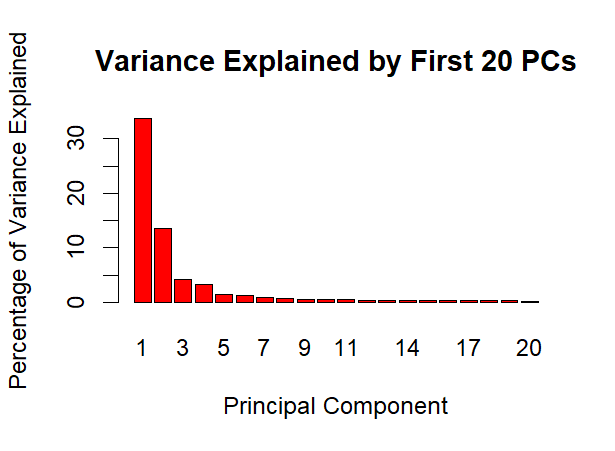
\includegraphics[keepaspectratio]{final PCA.png}}
\caption{pca}
\end{figure}
\end{block}
\end{frame}

\begin{frame}{5.UMAP Visualization:Generate a UMAP using a subset of
principal components you think are sufficiently informative. Justify
your choice of components in the report.}
\phantomsection\label{umap-visualizationgenerate-a-umap-using-a-subset-of-principal-components-you-think-are-sufficiently-informative.-justify-your-choice-of-components-in-the-report.}
\begin{block}{visualising the variance to choose the subset}
\phantomsection\label{visualising-the-variance-to-choose-the-subset}
var\_explained
\end{block}

\begin{block}{deciding on the 6th componment since it is the last higher
than 1}
\phantomsection\label{deciding-on-the-6th-componment-since-it-is-the-last-higher-than-1}
\end{block}

\begin{block}{running the UMAP}
\phantomsection\label{running-the-umap}
BiocManager::install(c(``scater'', ``scran'')) a library(scater) sce
\textless- runUMAP(sce, dimred = ``PCA'', n\_dimred = 6)

library(ggplot2) umap\_coords \textless- as.data.frame(reducedDim(sce,
``UMAP'')) colnames(umap\_coords) \textless- c(``UMAP1'', ``UMAP2'')
\end{block}

\begin{block}{plotting the UMAP}
\phantomsection\label{plotting-the-umap}
ggplot(umap\_coords, aes(x = UMAP1, y = UMAP2)) + geom\_point(size =
0.3, alpha = 1) + labs(title = ``UMAP Based on First 6 Principal
Components'') + theme\_minimal(12)

\begin{figure}
\centering
\pandocbounded{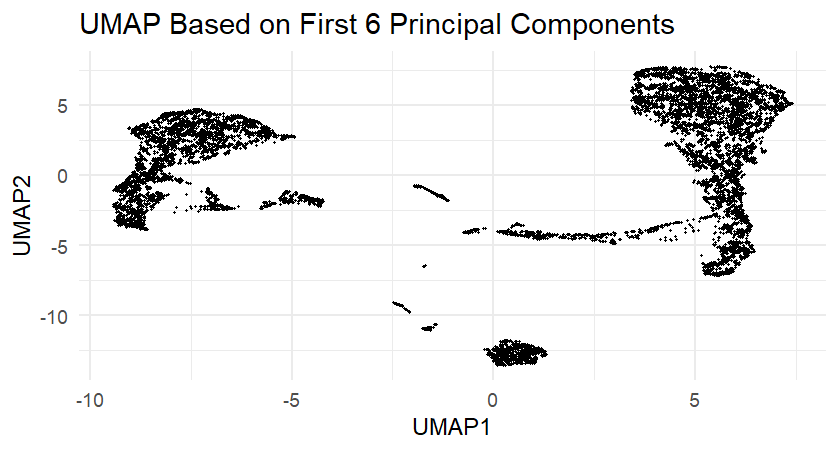
\includegraphics[keepaspectratio]{final UMAP.png}}
\caption{umap}
\end{figure}
\end{block}
\end{frame}

\begin{frame}{6.Clustering:Apply a clustering algorithm of your choice
and visualize the clusters. Clearly describe:The clustering method used,
Parameters and resolution settings, Interpretation of the resulting
clusters.Building shared nearest neighbor graph}
\phantomsection\label{clusteringapply-a-clustering-algorithm-of-your-choice-and-visualize-the-clusters.-clearly-describethe-clustering-method-used-parameters-and-resolution-settings-interpretation-of-the-resulting-clusters.building-shared-nearest-neighbor-graph}
library(SingleCellExperiment) library(scran) library(scater)
library(igraph) snn\_graph \textless-buildSNNGraph(sce, use.dimred =
``PCA'', k = 10)

\begin{block}{clustering with the Walktrap algorithm}
\phantomsection\label{clustering-with-the-walktrap-algorithm}
clusters \textless- igraph::cluster\_walktrap(snn\_graph)\$membership
\end{block}

\begin{block}{storing clusters in sce}
\phantomsection\label{storing-clusters-in-sce}
colLabels(sce) \textless- factor(clusters)

umap\_df \textless- as.data.frame(reducedDim(sce, ``UMAP''))
umap\_df\$Cluster \textless- colLabels(sce)
\end{block}

\begin{block}{plotting the UMAP based on the clusters found}
\phantomsection\label{plotting-the-umap-based-on-the-clusters-found}
library(ggplot2) ggplot(umap\_df, aes(x = UMAP1, y = UMAP2, color =
Cluster)) + geom\_point(size = 0.3, alpha = 1) + labs(title = ``UMAP
Colored by Clusters (Walktrap, k=10)'') + theme\_minimal(10)

\begin{figure}
\centering
\pandocbounded{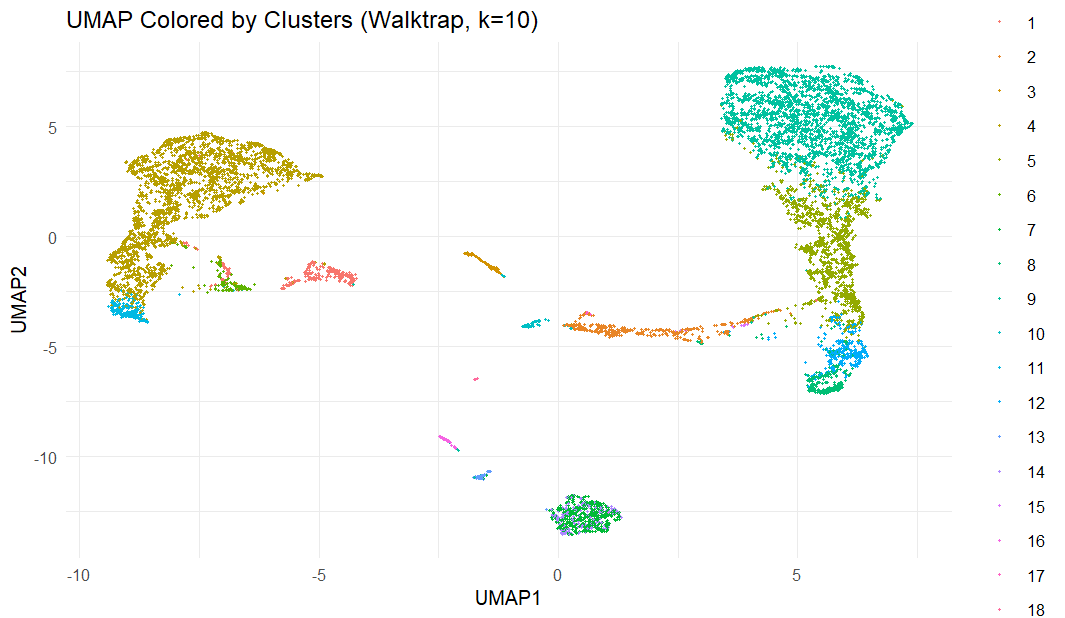
\includegraphics[keepaspectratio]{final clusters.png}}
\caption{clusters umap}
\end{figure}
\end{block}
\end{frame}

\begin{frame}{7.Cell Type Annotation:Using a cell annotation tool of
your choice annotate the dataset and discuss:Concordance or discordance
between clusters and predicted cell types,Evidence of heterogeneity or
homogeneity within clusters}
\phantomsection\label{cell-type-annotationusing-a-cell-annotation-tool-of-your-choice-annotate-the-dataset-and-discussconcordance-or-discordance-between-clusters-and-predicted-cell-typesevidence-of-heterogeneity-or-homogeneity-within-clusters}
\begin{block}{using sindleR}
\phantomsection\label{using-sindler}
BiocManager::install(``org.Hs.eg.db'') a \#\# selecting all
library(org.Hs.eg.db) library(SingleCellExperiment)
\end{block}

\begin{block}{loading reference dataset}
\phantomsection\label{loading-reference-dataset}
ensembl\_ids \textless- rownames(sce)
\end{block}

\begin{block}{removing version numbers}
\phantomsection\label{removing-version-numbers}
ensembl\_ids \textless- sub(``\textbackslash..*'', ``\,``, ensembl\_ids)
\end{block}

\begin{block}{mapping Ensembl to symbols}
\phantomsection\label{mapping-ensembl-to-symbols}
gene\_symbols \textless- mapIds( org.Hs.eg.db, keys = ensembl\_ids,
column = ``SYMBOL'', keytype = ``ENSEMBL'', multiVals = ``first'' )
\end{block}

\begin{block}{updating rownames}
\phantomsection\label{updating-rownames}
rownames(sce) \textless- gene\_symbols
\end{block}

\begin{block}{filtering out genes with NA}
\phantomsection\label{filtering-out-genes-with-na}
sce \textless- sce{[}!is.na(rownames(sce)), {]}
\end{block}

\begin{block}{running SingleR}
\phantomsection\label{running-singler}
library(celldex) library(SingleR) ref \textless-
celldex::HumanPrimaryCellAtlasData() pred \textless- SingleR(test = sce,
ref = ref, labels = ref\(label.main)
sce\)predicted\_cell\_type \textless- pred\$labels
\end{block}

\begin{block}{visualising the difference}
\phantomsection\label{visualising-the-difference}
library(ggplot2) umap\_df \textless-as.data.frame(reducedDim(sce,
``UMAP'')) umap\_df\(CellType <- sce\)predicted\_cell\_type

ggplot(umap\_df, aes(x = UMAP1, y = UMAP2, color = CellType)) +
geom\_point(size = 0.3, alpha = 1) + labs(title = ``UMAP Colored by
Predicted Cell Types'') + theme\_minimal(10)

\begin{figure}
\centering
\pandocbounded{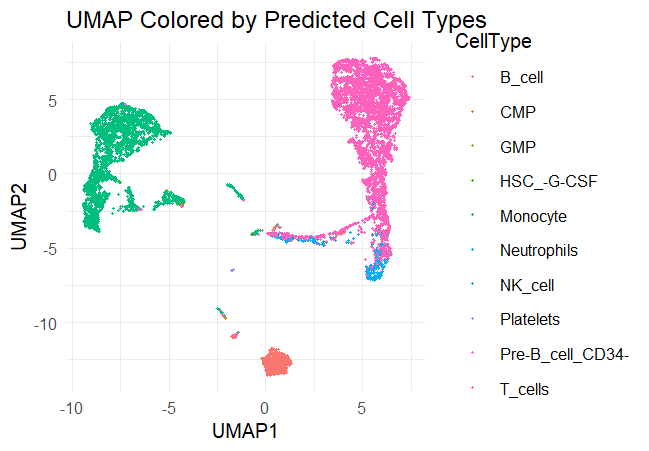
\includegraphics[keepaspectratio]{final UMAP by cell type.png}}
\caption{cell type umap}
\end{figure}
\end{block}
\end{frame}

\begin{frame}{8.Tissue Origin Inference:Based on gene markers,
annotation, and cluster structure, propose a hypothesis about the tissue
of origin for the dataset. Justify your guess with biological
reasoning.}
\phantomsection\label{tissue-origin-inferencebased-on-gene-markers-annotation-and-cluster-structure-propose-a-hypothesis-about-the-tissue-of-origin-for-the-dataset.-justify-your-guess-with-biological-reasoning.}
\begin{block}{ensuring both columns are clean}
\phantomsection\label{ensuring-both-columns-are-clean}
markers\_genes \textless- toupper(trimws(gtf\(gene_symbol))
panglao_genes <- toupper(trimws(panglao\)official.gene.symbol))
\end{block}

\begin{block}{matching by intersection}
\phantomsection\label{matching-by-intersection}
matched\_genes \textless- intersect(markers\_genes, panglao\_genes)
\end{block}

\begin{block}{filtering PanglaoDB by matched genes}
\phantomsection\label{filtering-panglaodb-by-matched-genes}
matched\_table \textless-
panglao{[}toupper(panglao\$official.gene.symbol) \%in\% matched\_genes,
{]}
\end{block}

\begin{block}{counting how many matched each cell type}
\phantomsection\label{counting-how-many-matched-each-cell-type}
celltype\_counts \textless-
as.data.frame(table(matched\_table\(cell.type))
celltype_counts <- celltype_counts[order(-celltype_counts\)Freq), {]}
print(celltype\_counts)
\end{block}

\begin{block}{plotting histogram}
\phantomsection\label{plotting-histogram}
library(ggplot2) colnames(celltype\_counts) \textless- c(``CellType'',
``Count'')

ggplot(celltype\_counts, aes(x = reorder(CellType, -Count), y = Count))
+ geom\_bar(stat = ``identity'', fill = ``purple'') + theme\_minimal() +
labs(title = ``Cell Type Frequency (from PanglaoDB markers)'', x =
``Cell Type'', y = ``Number of Marker Genes'') + theme(axis.text.x =
element\_text(angle = 45, hjust = 1))

\begin{figure}
\centering
\pandocbounded{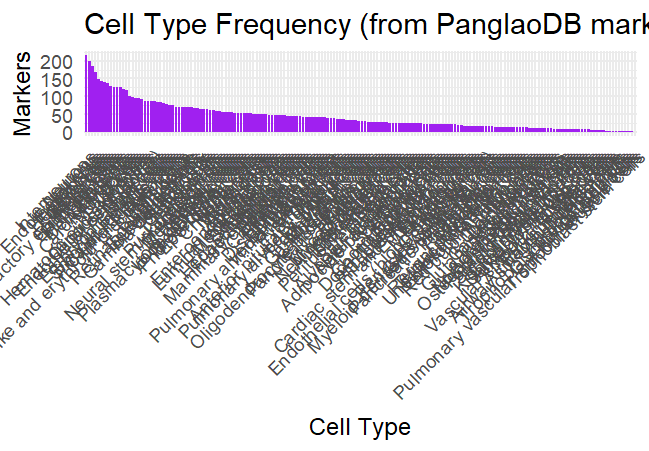
\includegraphics[keepaspectratio]{final tissue.png}}
\caption{tissues}
\end{figure}
\end{block}

\begin{block}{they are too much to visualise, let's see the top 25
tissues}
\phantomsection\label{they-are-too-much-to-visualise-lets-see-the-top-25-tissues}
library(ggplot2)
\end{block}

\begin{block}{selecting top 25 most frequent cell types}
\phantomsection\label{selecting-top-25-most-frequent-cell-types}
top25 \textless-head(celltype\_counts{[}order(-celltype\_counts\$Count),
{]}, 25)
\end{block}

\begin{block}{plotting histogram}
\phantomsection\label{plotting-histogram-1}
ggplot(top25, aes(x = reorder(CellType, -Count), y = Count)) +
geom\_bar(stat = ``identity'', fill = ``yellow'') + theme\_minimal() +
labs(title = ``Top 25 Cell Types by Marker Frequency'', x = ``Cell
Type'', y = ``Number of Marker Genes'') + theme(axis.text.x =
element\_text(angle = 45, hjust = 1))

\begin{figure}
\centering
\pandocbounded{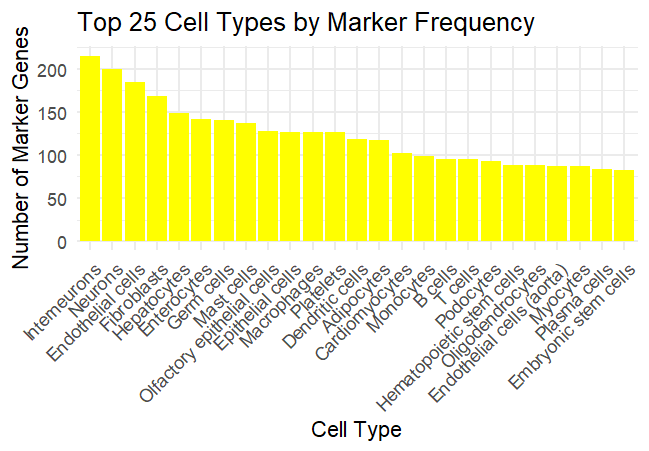
\includegraphics[keepaspectratio]{top 25 tissues.png}}
\caption{top 25 tissues}
\end{figure}
\end{block}
\end{frame}

\end{document}
